\documentclass[tikz]{standalone}
\usetikzlibrary{calc}
\usepackage{pgfplots}

\begin{document}


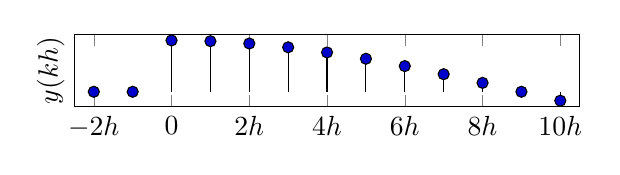
\begin{tikzpicture}
\begin{axis}[ width=8cm,
  height=2.5cm,
  %xlabel={$t$},
  ylabel={$y(kh)$},
  xtick = {-2, 0, 2, 4, 6, 8, 10},
  xticklabels={$-2h$, $0$, $2h$, $4h$, $6h$, $8h$, $10h$},
  ytick=\empty,
  xmin=-2.5,
  xmax=10.5,
]

\addplot+[black, ycomb, domain=-2:10, samples=13,variable=k] { (k>=0)*cos(10*k)}; 

\end{axis}
\end{tikzpicture}
\end{document}
